%%% LaTeX Template: Newsletter
%%%
%%% Source: http://www.howtotex.com/
%%% Feel free to distribute this template, but please keep the referal to HowToTeX.com.
%%% Date: September 2011


%%% ---------------
%%% PREAMBLE
%%% ---------------
\documentclass[10pt,a4paper]{article}

% Define geometry (without using the geometry package)
\setlength\topmargin{-48pt}
\setlength\headheight{0pt}
\setlength\headsep{25pt}
\setlength\marginparwidth{-20pt}
\setlength\textwidth{7.0in}
\setlength\textheight{9.5in}
\setlength\oddsidemargin{-30pt}
\setlength\evensidemargin{-30pt}

\frenchspacing						% better looking spacing

% Call packages we'll need
\usepackage[english]{babel}			% english
\usepackage{graphicx}				% images
\usepackage{amssymb,amsmath}		% math
\usepackage{multicol}				% three-column layout
\usepackage{url}					% clickable links
\usepackage{marvosym}				% symbols
\usepackage{wrapfig}				% wrapping text around figures
\usepackage[T1]{fontenc}			% font encoding
\usepackage{charter} 				% Charter font for main content
\usepackage{blindtext}				% dummy text
\usepackage{datetime}				% custom date
\usepackage{caption}
	\newdateformat{mydate}{\monthname[\THEMONTH] \THEYEAR}
\usepackage[pdfpagemode=FullScreen,
			colorlinks=false]{hyperref}	% links and pdf behaviour

% Customize (header and) footer
\usepackage{fancyhdr}
\pagestyle{fancy}
\lfoot{	\footnotesize 
		Newletter from LifeguardRobotics.com \\
		\Mundus\ \href{http://www.lifeguardrobotics.com}{LifeguardRobotics.com}	\quad
		\Telefon\ (831) 704-6771										\quad
		\Letter\ \href{mailto:lifeguardrobotics@gmail.com}{lifeguardrobotics@gmail.com}
	  }
\cfoot{}
\rfoot{\footnotesize ~\\ Page \thepage}
\renewcommand{\headrulewidth}{0.0pt}	% no bar on top of page
\renewcommand{\footrulewidth}{0.4pt}	% bar on bottom of page

%%% ---------------
%%% DEFINITIONS
%%% ---------------

% Define separators
\newcommand{\HorRule}[1]{\noindent\rule{\linewidth}{#1}} % Creating a horizontal rule
\newcommand{\SepRule}{\noindent							 % Creating a separator
						\begin{center}
							\rule{250pt}{1pt}
						\end{center}
						}						

% Define Title en News input
\newcommand{\JournalName}[1]{%
		\begin{center}	
			\Huge \usefont{T1}{cmr}{m}{n}
			#1%
		\end{center}	
		\par \normalsize \normalfont}
		
\newcommand{\JournalIssue}[1]{%
        \hfill \textsc{\mydate \today, No #1}
        \par \normalsize \normalfont}

\newcommand{\NewsItem}[1]{%
		\usefont{T1}{augie}{m}{n} 	
		\large #1 \vspace{4pt}
		\par \normalsize \normalfont}
		
\newcommand{\NewsAuthor}[1]{%
			\hfill by \textsc{#1} \vspace{4pt}
			\par \normalfont}		


%%% ---------------
%%% BEGIN DOCUMENT
%%% ---------------
\begin{document}
% Title	
% -----
\JournalIssue{2}
\JournalName{The Autonomous Lifeguard Project}
\noindent\HorRule{3pt} \\[-0.75\baselineskip]
\HorRule{1pt}
% -----

% Front article
% -----
\vspace{0.5cm}
	\SepRule
\vspace{0.5cm}
\begin{center}
\begin{minipage}[h]{0.80\linewidth}
	\begin{wrapfigure}{l}{0.378\textwidth}
		{%
		\setlength{\fboxsep}{0pt}%
		\setlength{\fboxrule}{1pt}%
		\fbox{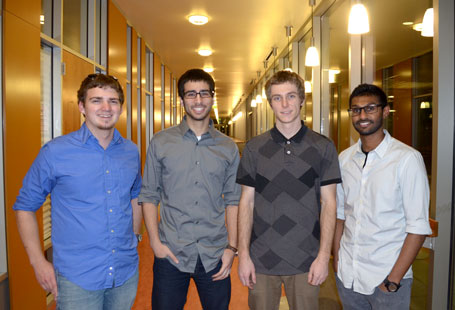
\includegraphics[width=0.39\textwidth]{al-group.jpg}}%
		\caption*{Left to right: J. Ash, S. Dajani, D. Goodman, D. Deo}
		}%
		%\\	% this spacer is needed to make the text on the right fit OK
	\end{wrapfigure}
	
	\NewsItem{Who Are We}
	\emph{We are a group of UC Santa Cruz computer and robotics engineering students who are building a robot to assist lifeguards in saving drowning individuals on beaches, at sea, and in other bodies of water. In the United States, there has been a reported 99 people that have drowned in the past year alone, with a good number of them occurring while a lifeguard was on duty. We propose an autonomous boat that can navigate to a person, allowing them to hang on and stay a float until the lifeguard arrives. Our aim is to keep beaches safer by reducing the risk of drowning.}
\end{minipage}
\end{center}
% -----


% 
% -----
\vspace{0.5cm}
	\SepRule
\vspace{0.5cm}
\begin{multicols}{3}
	\NewsItem{Milestones}
	\NewsAuthor{D. Goodman}
    
    We are all very pleased to announce that our command center is nearing completion. As March comes to an end, our project continues to grow and progress. Throughout this month, many hours were dedicated to implementing and integrating sensors, performing testing, and debugging the command center. Last week, we met our desired basic functionality for the command center, and created a video demonstrating its usage. A technical presentation was given before an audience of our peers that discussed our progress, challenges, and future plans.
\begin{center}
			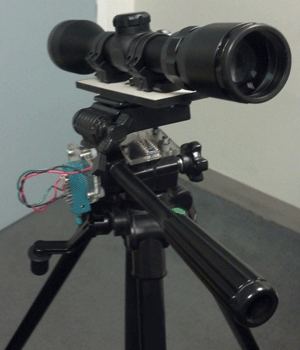
\includegraphics[width=0.63\linewidth]{cc.png}
		\end{center}
The months of February and March have brought our team closer to reaching our goals. The completion of our boat is the next major milestone. We plan to accomplish this during April and May, so that by June we will have a working prototype. 
		
% -----

\vspace{1cm}
% Other news (2)
% -----
\NewsItem{Future Work}
\NewsAuthor{D. Goodman}
	Although the engineering buildings are very quiet during spring break, we are currently working hard to get the boat into the water. Shehadeh is working diligently to equip the boat with the new motors and emergency RC receiver. These modifications will allow us to reach a drowning victim quickly, and safely. Darrel, David, and John are busy implementing autonomous features into the boat, via a navigation and drive system. Our goal is to have the boat navigating on its own in the water by this coming weekend.

Following this weekend's testing, we will continue to work on the navigation system, and to get the command center talking to the boat from the shore. Once the boat is able to navigate to waypoints, we will begin the integration of our human detection sensor array, which includes sonar and thermal imaging. We are eager to continue making progress in every direction, and spring is proving to be very productive so far.

% -----
%\columnbreak
\vspace{1cm}
% Other news (2)
% -----
\NewsItem{Support}
\NewsAuthor{D. Deo}
The Autonomous Lifeguard Group is moving quite swiftly and is hopeful that the next phases of the project will yield exceptional results. As a devoted team, we are currently funding the project entirely ourselves. Optimistic about the future of the Autonomous Lifeguard Project, we would appreciate any form of support that would help the project advance. Donations are welcome and can be submitted via our website. All considerations will be recognized by the team.
\end{multicols}
% -----
\end{document} 

